Il periodo di Progettazione di dettaglio e codifica inizia con la consegna della RP e termina con la consegna della RQ.\newline
Durante questo periodo, vengono svolte le seguenti attività:
\begin{itemize}
	\item \textbf{Incremento: }modifiche incrementali ai seguenti documenti, ove necessario:
	\begin{itemize}
		\item Analisi dei requisiti;
		\item Piano di progetto;
		\item Piano di qualifica;
		\item Glossario;
		\item Norme di progetto;
		\item Specifica Tecnica;
	\end{itemize}
	\item \textbf{Product Baseline: }sulla base della specifica tecnica viene redatto il documento di definizione di prodotto, nella quale sono contenute le scelte progettuali di dettaglio;
	\item \textbf{Codifica: }basandosi sulla definizione di prodotto, viene scritto il codice sorgente;
	\item \textbf{Manuale Utente: }redazione del manuale utente del prodotto. 
\end{itemize}


\begin{figure}[H]
	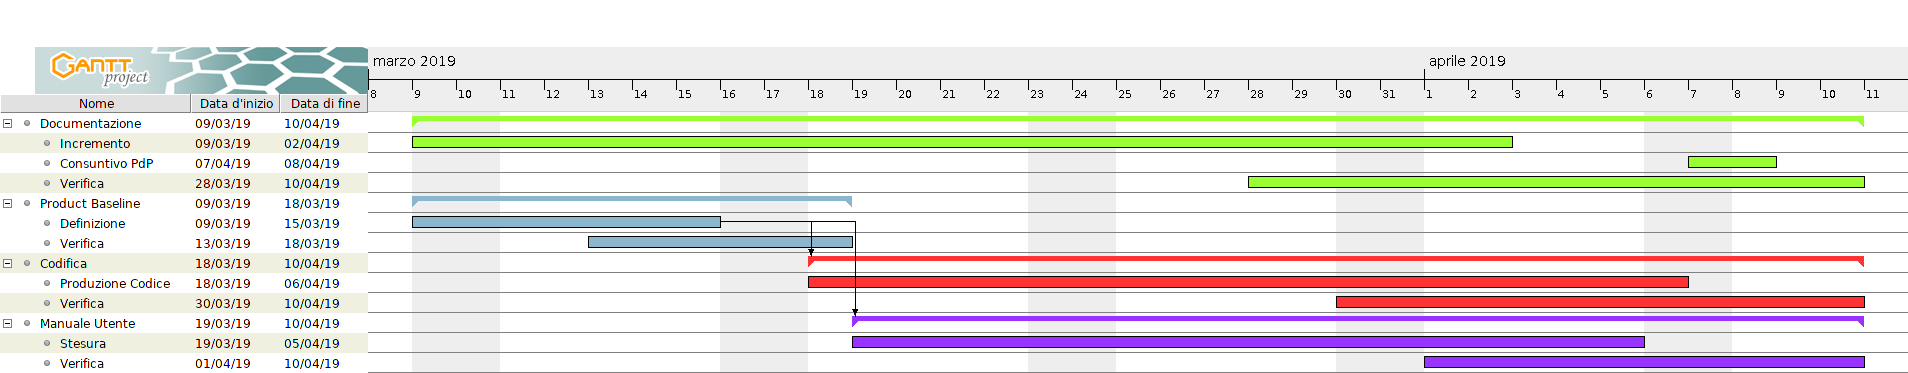
\includegraphics[width=1\linewidth]{Pianificazione/Progettazione_Dettaglio_Codififca.png}
	\caption{Diagramma di Gantt del periodo di Progettazione di dettaglio e codifica}
\end{figure}